In the previous chapter a set of suggestions for improving a BPMN diagram where listed. As it was also mentioned, only a fraction of these improvements can be automated. 

This chapter will provide a example how the mentioned not automatable and automatable suggestions can be applied together to an existing BPMN model. 

At first, the example BPMN model used for this case study and the evaluation that is done by the software on this BPMN will be explained. After that, the suggestions as they are listed in section \ref{last} will be implemented one by one, using the software evaluation as aid. 

In the end, the original BPMN will be compared with the final result using quantitive emasues as described in section \ref{quant}.

\section{The example model}
The used BPMN model for this chapter will be a client registration process which is a real live process used in the telecommunication filed that was changed in order to be used in this thesis. The graphical representation of the process model can be found in figure \ref{fig:example-process} and the full XML structure is in the appendix section \ref{app-1}

\begin{figure}[H]
	\centering
	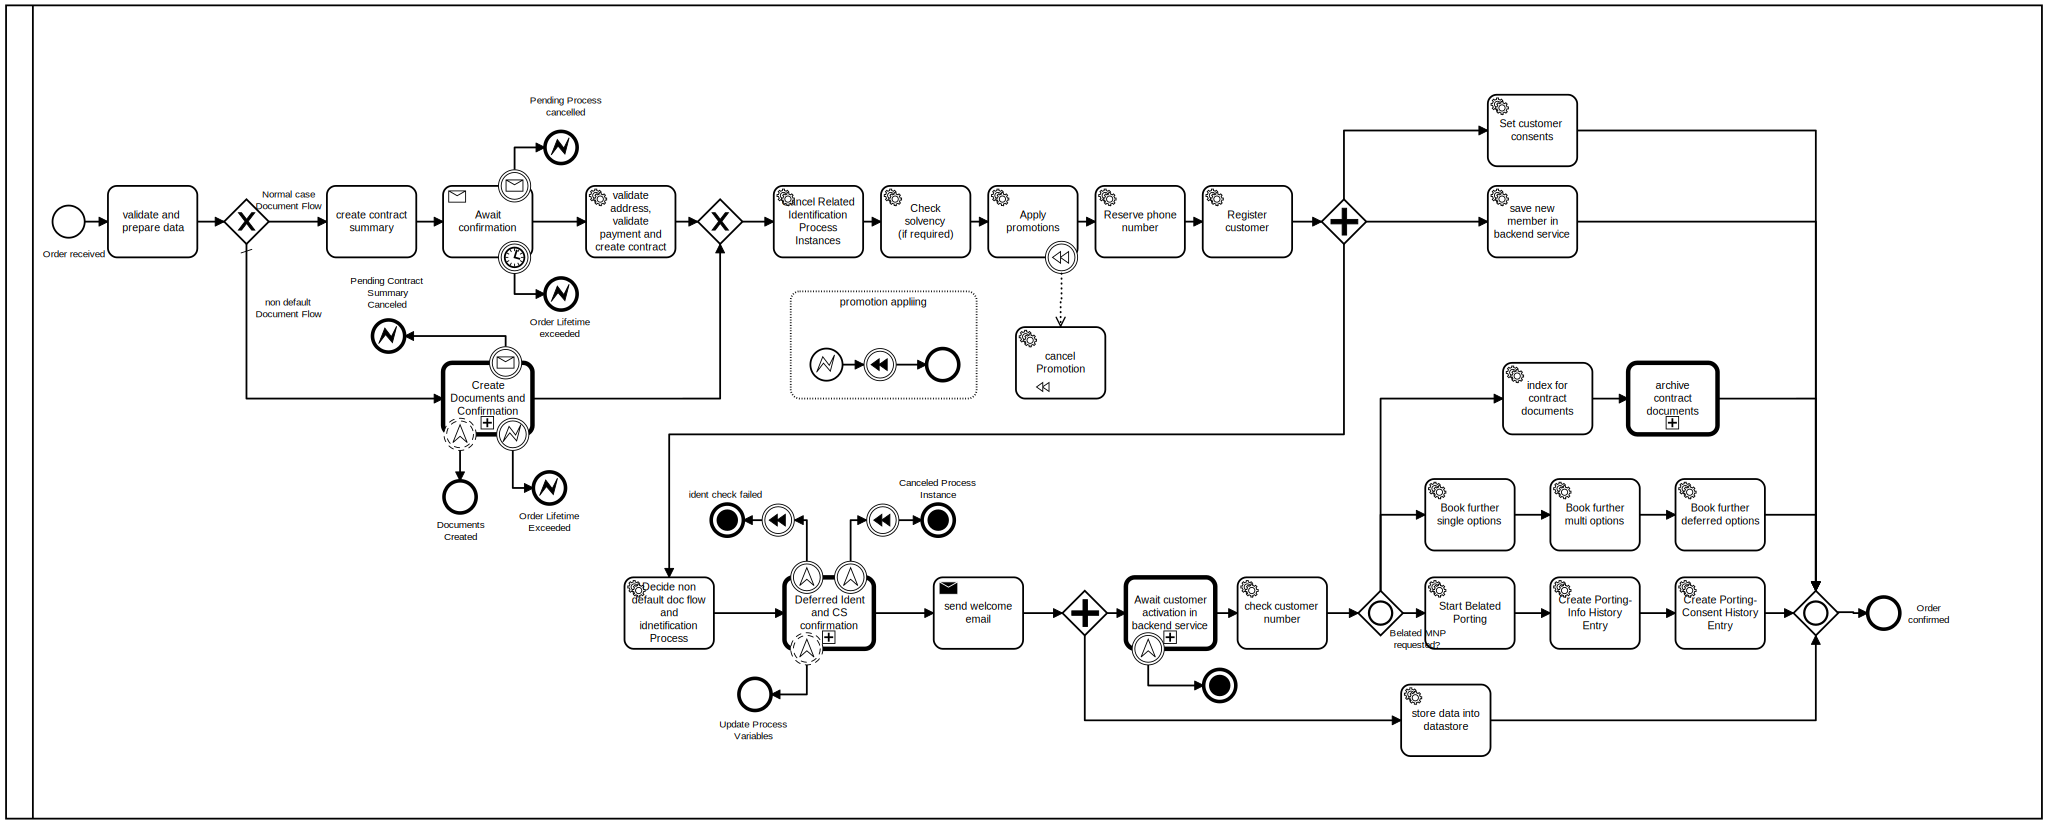
\includegraphics[width=1.7\columnwidth, angle=90 ]{graphics/process-bpmn.pdf}
	\caption{Example of a process where tasks can be merged together} 
	\label{fig:example-process} 
\end{figure}

\section{Evaluation by the Software}
In order to evaluate the best practices that where automated by the software as mentioned in section \ref{last}, the BPMN Model was given as input for the software. The full output can be found in section \ref{app-1} the following output for each Suggestion/Rule was given:
\paragraph{Comply with Naming Conventions}~\\
As described in chapter \ref{naming-con}, this algorithm scans the BPMN model for events, tasks or gateways that have more than five words in their label. The following list of elements is returned that violate this rule:
\begin{lstlisting}[language=json]
"effectedElements": [
{
	"id": "ServiceTask_DefaultDocWorkflowPostAwaitConfirmation",
	"name": "validate address, validate payment and create contract",
	"type": "Task"
},
{
	"id": "DecideIdAndCsProcess",
	"name": "Decide non default doc flow and idnetification Process",
	"type": "Task"
},
{
	"id": "save_member_for_riskident",
	"name": "save new member in backend service",
	"type": "Task"
}
\end{lstlisting}


\paragraph{Eliminate Manual Tasks}~\\
When searching for manual tasks in the process (see section \ref{soft-manual}), only one can be identified and is returned:
\begin{lstlisting}[language=json]
"effectedElements": [
{
	"id": "data_to_warehouse",
	"name": "store data into datastore",
	"type": "Task"
}
\end{lstlisting}
\paragraph{No two consecutive Tasks handled by the same resource}~\\
Another rule that was implemented was that no two consecutive tasks should be processed by the same resource. The Software identified the following tasks that could be merged with its successor:
\begin{lstlisting}[language=json]
"effectedElements": [
{
	"id": "CancelRelatedWebIdent",
	"name": "Cancel Related Identification Process Instances",
	"type": "Task"
},
{
	"id": "ReserveMsisdn",
	"name": "Reserve phone number",
	"type": "Task"
},
{
	"id": "BookAutoTopups",
	"name": "Book further multi options",
	"type": "Task"
},
{
	"id": "ServiceTask_0p0tajd",
	"name": "Start Belated Porting",
	"type": "Task"
},
{
	"id": "ServiceTask_0e2r82f",
	"name": "Create Porting-Info History Entry",
	"type": "Task"
},
{
	"id": "BookSingleTopups",
	"name": "Book further single options",
	"type": "Task"
}
]
\end{lstlisting}
\paragraph{Inclusive Gateways over combining parallel and exclusive Gateways}~\\
As described in section \ref{inc-sw} it is preferred to use inclusive gateways instead of combining parallel and exclusive gateways. The only element that violates that rule in the given BPMN is returned:
\begin{lstlisting}[language=json]
"effectedElements": [
{
	"id": "ParallelGateway_0crudor",
	"name": null,
	"type": "Gateway"
}
]
\end{lstlisting}
\section{Comply with Naming Conventions}
%TODO
%see  https://docs.camunda.io/docs/components/best-practices/modeling/creating-readable-process-models/
%   & https://docs.camunda.io/docs/components/best-practices/modeling/naming-bpmn-elements/
\subsection{renaming tasks}
\subsection{renaming gateways}
\subsection{rename events}

\section{Extend automation boundaries}
%TODO

\section{Eliminate Manual Tasks}
%TODO

\section{Complete the process model}
%TODO

\section{No two consecutive Tasks handled by the same resource}
%TODO

\section{Inclusive Gateways over combining parallel and exclusive Gateways}
%TODO

\section{Value Added Analysis}
%TODO

\section{Evaluate Suggestions Quantitative}
%TODO

